\chapter{Background}
\label{cha:bkg}
%Literature Review
This chapter provides the readers with detailed biology background of object recognition in the brain and with the fundamental principles of neural modelling using spiking neural networks.
This is followed by an introduction to the neuromorphic hardware platform specialised for neural simulations of visual processing.

\section{How the Brain Represent Objects?}
\label{sec:bio}
The central visual system consists of several cortical areas responsible for visual processing, which are placed in a hierarchical pattern according to the anatomical experiments~\cite{felleman1991distributed}.
There are two basic streams locating in the visual area: a dorsal and a ventral pathway (Figure [???]).
They differ in behavioural patterns according to the observation from brain lesions~\cite{prado2005two}, and also in functions where the dorsal pathway targets on the `where' tasks and the ventral on the `what'.
The ventral (`what') visual stream holds the critical circuits for object recognition and stimulus identification, whereas the dorsal pathway (`where') pathway contributes to the processing of the spatial location of the stimulus~\cite{prado2005two, Ungerleider1994157}.
Another definition of the difference between these two pathways is a `perception/action' dichotomy: the ventral stream, `perception' pathway, cognises the world by means of object recognition and memory, while the dorsal stream, `action' pathway, provides real-time visual guidance for motor actions such as eye movements and grasping objects~\cite{goodale1992separate}. 

This research mainly focuses on the ventral visual pathway, since it dominates the object recognition among the cortical areas.
Thus, the dorsal pathway will beyond the scope of the this study. 


\subsection{The Ventral Visual Pathway}
Decades of evidence argue that
the primate ventral visual processing
stream—a set of cortical areas arranged
along the occipital and temporal lobes
(Figure 3A)—houses key circuits that underlie object recognition
behavior.
The ventral visual stream has been parsed into distinct visual
‘‘areas’’ based on anatomical connectivity patterns, distinctive anatomical structure, and retinotopic mapping (Felleman and
Van Essen, 1991). Complete retinotopic maps have been re-
vealed for most of the visual field (at least 40 degrees eccentricity
from the fovea) for areas V1, V2, and V4 (Felleman and Van Es-
sen, 1991) and thus each area can be thought of as conveying
a population-based re-representation of each visually presented
image. Within the IT complex, crude retinotopy exists over the
more posterior portion (pIT; Boussaoud et al., 1991; Yasuda
et al., 2010), but retinotopy is not reported in the central and
anterior regions (Felleman and Van Essen, 1991). Thus, while
IT is commonly parsed into subareas such as TEO and TE (Jans-
sen et al., 2000; Saleem et al., 2000, 1993; Suzuki et al., 2000;
Von Bonin and Bailey, 1947) or posterior IT (pIT), central IT
(cIT), and anterior IT (aIT) (Felleman and Van Essen, 1991), it is
unclear if IT cortex is more than one area, or how the term
‘‘area’’ should be applied.
a hierarchical
organization (as opposed to a parallel or fully interconnected
organization) of the areas with visual information traveling first
from the retina to the lateral geniculate nucleus of the thalamus
(LGN), and then through cortical area V1 to V2 to V4 to IT (Felle-
man and Van Essen, 1991). Consistent with this, the (mean) first
visually evoked responses of each successive cortical area are
successively lagged by about 10 ms (Nowak and Bullier, 1997;
Schmolesky et al., 1998; see Figure 3B). Thus, just around 100 ms after
image photons impinge on the retina, a first wave of image-
selective neuronal activity is present throughout much of IT
(e.g., Desimone et al., 1984; DiCarlo and Maunsell, 2000; Hung
et al., 2005; Kobatake and Tanaka, 1994a; Logothetis and Shein-
berg, 1996; Tanaka, 1996).

V1\\
V2\\
V4\\
IT- the main part. including IT single neuron behaviour.\\
%PFC
\subsection{Neural Code for Object Representation}
%\subsection{Untangling Object Representation}
%A graphical intuition into the Problem.
we consider the neuronal representation in a given
cortical area (e.g., the ‘‘IT representation’’) to be the spatio-temporal pattern of spikes produced by the set of pyramidal neurons
that project out of that area (e.g., the spiking patterns traveling
along the population of axons that project out of IT; see
Figure 3B). How is the spiking activity of individual neurons
thought to encode visual information?

Single neuron representation\\
Most studies have investigated the response properties of
neurons in the ventral pathway by assuming a firing rate (or,
equivalently, a spike count) code, i.e., by counting how many
spikes each neuron fires over several tens or hundreds of milli-
seconds following the presentation of a visual image, adjusted
for latency (e.g., see Figures 4A and 4B). Historically, this
temporal window (here called the ‘‘decoding’’ window) was justi-
fied by the observation that its resulting spike rate is typically well
modulated by relevant parameters of the presented visual
images (such as object identity, position, or size; Desimone
et al., 1984; Kobatake and Tanaka, 1994b; Logothetis and
Sheinberg, 1996; Tanaka, 1996) (see examples of IT neuronal
responses in Figures 4A–4C), analogous to the well-understood
firing rate modulation in area V1 by ‘‘low level’’ stimulus
properties such as bar orientation (reviewed by Lennie and Mov-
shon, 2005).

population coding\\
Like all cortical neurons, neuronal spiking throughout the
ventral pathway is variable in the ms-scale timing of spikes, re-
sulting in rate variability for repeated presentations of a nominally
identical visual stimulus. This spike timing variability is consistent
with a Poisson-like stochastic spike generation process with an
underlying rate determined by each particular image (e.g., Kara
et al., 2000; McAdams and Maunsell, 1999). Despite this vari-
ability, one can reliably infer what object, among a set of tested
visual objects, was presented from the rates elicited across the
IT population (e.g., Abbott et al., 1996; Aggelopoulos and Rolls,
2005; De Baene et al., 2007; Heller et al., 1995; Hung et al., 2005;
Li et al., 2009; Op de Beeck et al., 2001; Rust and DiCarlo, 2010).
It remains unknown whether the ms-scale spike variability found
in the ventral pathway is ‘‘noise’’ (in that it does not directly help
stimulus encoding/decoding) or if it is somehow synchronized
over populations of neurons to convey useful, perhaps ‘‘multi-plexed’’ information (reviewed by Ermentrout et al., 2008).

50 ms window matters\\
IT neuronal spiking patterns (e.g., concatenated decoding
windows, each less than 50 ms) does not convey significantly
more information about object identity than larger time windows
(e.g., a single, 200 ms decoding window), suggesting that the
results of ventral stream processing are well described by a firing
rate code where the relevant underlying time scale is 50 ms
(Abbott et al., 1996; Aggelopoulos and Rolls, 2005; Heller
et al., 1995; Hung et al., 2005). While different time epochs rela-
tive to stimulus onset may encode different types of visual infor-
mation (Brincat and Connor, 2006; Richmond and Optican,
1987; Sugase et al., 1999), very reliable object information is
usually found in IT in the first 50 ms of neuronal response
(i.e., 100–150 ms after image onset, see Figure 4A). More specif-
ically, (1) the population representation is already different for
different objects in that window (DiCarlo and Maunsell, 2000),
and (2) responses in that time window are more reliable because
peak spike rates are typically higher than later windows (e.g.,
Hung et al., 2005).

\subsection{IT}
simple weighted summations of IT spike\\
Although visual information processing in the first stage of the
ventral stream (V1) is reasonably well understood (see Lennie
and Movshon, 2005 for review), processing in higher stages
(e.g., V4, IT) remains poorly understood. Nevertheless, we
know that the ventral stream produces an IT pattern of activity
that can directly support robust, real-time visual object catego-
rization and identification, even in the face of changes in object
position and scale, limited clutter, and changes in background
context (Hung et al., 2005; Li et al., 2009; Rust and DiCarlo,
2010). Specifically, simple weighted summations of IT spike
counts over short time intervals (see section 2) lead to high rates
of cross-validated performance for randomly selected popula-
tions of only a few hundred neurons (Hung et al., 2005; Rust
and DiCarlo, 2010) (Figure 4E), and a simple IT weighted sum-
mation scheme is sufficient to explain a wide range of human
invariant object recognition behavior (Majaj et al., 2012).

Better than lower level\\
Importantly, IT neuronal populations are demonstrably better
at object identification and categorization than populations
at earlier stages of the ventral pathway (Freiwald and Tsao,
2010; Hung et al., 2005; Li et al., 2009; Rust and DiCarlo,
2010).

A Contemporary View of IT Single Neurons\\
Respond to different variations\\
How do these IT neuronal population phenomena (above)
depend on the responses of individual IT neurons? Under-
standing IT single-unit responses has proven to be extremely
challenging and while some progress has been made (Brincat
and Connor, 2004; Yamane et al., 2008), we still have a poor
ability to build encoding models that predict the responses of
each IT neuron to new images (see Figure 4B). Nevertheless,
we know that IT neurons are activated by at least moderately
complex combinations of visual features (Brincat and Connor,
2004; Desimone et al., 1984; Kobatake and Tanaka, 1994b; Per-
rett et al., 1982; Rust and DiCarlo, 2010; Tanaka, 1996) and that
they are often able to maintain their relative object preference
over small to moderate changes in object position and size (Brin-
cat and Connor, 2004; Ito et al., 1995; Li et al., 2009; Rust and
DiCarlo, 2010; Tove ́e et al., 1994), pose (Logothetis et al.,
1994), illumination (Vogels and Biederman, 2002), and clutter
(Li et al., 2009; Missal et al., 1999, 1997; Zoccolan et al., 2005).

respond to more objects\\
Contrary to popular depictions of IT neurons as narrowly
selective ‘‘object detectors,’’ neurophysiological studies of IT
are in near universal agreement with early accounts that describe
a diversity of selectivity: ‘‘We found that, as in other visual areas, most IT neurons respond to many different visual stimuli and,
thus, cannot be narrowly tuned ‘detectors’ for particular
complex objects.’’ (Desimone et al., 1984). For example,
studies that involve probing the responses of IT cells with large
and diverse stimulus sets show that, while some neurons appear
highly selective for particular objects, they are the exception not
the rule. Instead, most IT neurons are broadly tuned and the
typical IT neuron responds to many different images and objects
(Brincat and Connor, 2004; Freedman et al., 2006; Kreiman et al.,
2006; Logothetis et al., 1995; Op de Beeck et al., 2001; Rolls,
2000; Rolls and Tovee, 1995; Vogels, 1999; Zoccolan et al.,
2007; see Figure 4B).

conclusion\\
Such findings argue for a distributed representation of visual
objects in IT, as suggested previously (e.g., Desimone et al.,
1984; Kiani et al., 2007; Rolls and Tovee, 1995)—a view that
motivates the population decoding approaches described
above (Hung et al., 2005; Li et al., 2009; Rust and DiCarlo,
2010). That is, single IT neurons do not appear to act as sparsely
active, invariant detectors of specific objects, but, rather, as
elements of a population that, as a whole, supports object recog-
nition. This implies that individual neurons do not need to be
invariant. Instead, the key single-unit property is called neuronal
‘‘tolerance’’: the ability of each IT neuron to maintain its prefer-
ences among objects, even if only over a limited transformation
range (e.g., position changes; see Figure 4C; Li et al., 2009).
Mathematically, tolerance amounts to separable single-unit
response surfaces for object shape and other object variables
such as position and size (Brincat and Connor, 2004; Ito et al.,
1995; Li et al., 2009; Tove ́e et al., 1994; see Figure 4D). This
contemporary view, that neuronal tolerance is the required and
observed single-unit phenomenology, has also been shown for
less intuitive identity-preserving transformations such as the
addition of clutter (Li et al., 2009; Zoccolan et al., 2005).


Summery\\
Taken together, the neurophysiological evidence can be
summarized as follows. First, spike counts in 50 ms IT decod-
ing windows convey information about visual object identity.
Second, this information is available in the IT population begin-
ning 100 ms after image presentation (see Figure 4A). Third,
the IT neuronal representation of a given object across changes
in position, scale, and presence of limited clutter is untangled
from the representations of other objects, and object identity can
be easily decoded using simple weighted summation codes (see
Figures 2B, 4D, and 4E). Fourth, these codes are readily
observed in passively viewing subjects, and for objects that
have not been explicitly trained (Hung et al., 2005). In sum, our
view is that the ‘‘output’’ of the ventral stream is reflexively ex-
pressed in neuronal firing rates across a short interval of time
(50 ms) and is an ‘‘explicit’’ object representation (i.e., object
identity is easily decodable), and the rapid production of this
representation is consistent with a largely feedforward, nonlinear
processing of the visual input.
\subsection{Hierarchical Abstractions}
Feed-forward, hierarchical organisation and abstraction.


We have arrived at a putative canonical meta job description,
local subspace untangling, by working our way ‘‘top-down’’
from the overall goal of visual recognition and considering neuro-
anatomical data. How might local subspace untangling be
instantiated within neuronal circuits and single neurons?
Historically, mechanistic insights into the computations per-
formed by local cortical circuits have derived from ‘‘bottom-up’’approaches that aim to quantitatively describe the encoding
functions that map image features to the firing rate responses
of individual neurons. One example is the conceptual encoding
models of Hubel and Wiesel (1962), which postulate the existence
of two operations in V1 that produce the response properties of
the ‘‘simple’’ and ‘‘complex’’ cells. First, V1 simple cells imple-
ment AND-like operations on LGN inputs to produce a new
form of ‘‘selectivity’’—an orientation-tuned response. Next, V1
complex cells implement a form of ‘‘invariance’’ by making OR-
like combinations of simple cells tuned for the same orientation.
These conceptual models are central to current encoding
models of biological object recognition (e.g., Fukushima, 1980;
Riesenhuber and Poggio, 1999b; Serre et al., 2007a), and they
have been formalized into the linear-nonlinear (LN) class of en-
coding models in which each neuron adds and subtract its inputs,
followed by a static nonlinearity (e.g., a threshold) to produce
a firing rate response (Adelson and Bergen, 1985; Carandini
et al., 2005; Heeger et al., 1996; Rosenblatt, 1958). While LN-style
models are far from a synaptic-level model of a cortical circuit,
they are a potentially powerful level of abstraction in that they
can account for a substantial amount of single-neuron response
patterns in early visual (Carandini et al., 2005), somatosensory
(DiCarlo et al., 1998), and auditory cortical areas (Theunissen
et al., 2000). Indeed, a nearly complete accounting of early level
neuronal response patterns can be achieved with extensions to
the simple LN model framework—most notably, by divisive
normalization schemes in which the output of each LN neuron
is normalized (e.g., divided) by a weighted sum of a pool of nearby
neurons (reviewed by Carandini and Heeger, 2011). Such
schemes were used originally to capture luminance and contrast
and other adaptation phenomena in the LGN and V1 (Mante et al.,
2008; Rust and Movshon, 2005), and they represent a broad class
of models, which we refer to here as the ‘‘normalized LN’’ model
class (NLN; see Figure 5).
We do not know whether the NLN class of encoding models
can describe the local transfer function of any output neuron at
any cortical locus (e.g., the transfer function from a V4 subpop-
ulation to a single IT neuron). However, because the NLN model
is successful at the first sensory processing stage, the parsimo-
nious view is to assume that the NLN model class is sufficient but
that the particular NLN model parameters (i.e., the filter weights,
the normalization pool, and the specific static nonlinearity) of
each neuron are uniquely elaborated. Indeed, the field has
implicitly adopted this view with attempts to apply cascaded
NLN-like models deeper into the ventral stream (e.g., David
et al., 2006). Unfortunately, the approach requires exponentially
more stimulus-response data to try to constrain an exponentially
expanding set of possible cascaded NLN models, and thus we cannot yet distinguish between a principled inadequacy of the
cascaded NLN model class and a failure to obtain enough
data. This is currently a severe ‘‘in practice’’ inadequacy of the
cascaded NLN model class in that its effective explanatory
power does not extend far beyond V1 (Carandini et al., 2005).
Indeed, the problem of directly determining the specific image-
based encoding function (e.g., a particular deep stack of NLN
models) that predicts the response of any given IT neuron
(e.g., the one at the end of my electrode today) may be practically
impossible with current methods.

\section{Spiking Neural Network}
\label{sec:pgr}
%All the literature review I can borrow from the previous report.
\subsection{Neuronal Model}
\subsubsection{The Membrane Potential}
A typical neuron is divided into three parts: the dendrites, the soma and the axon. Generally speaking, the dendrites receive the input signals from the previous neurons. The soma is where the received input signals are being processed and the axon is where the output signals are transmitted. The synapse is between every two neurons; if a neuron j sends a signal across the synapse to neuron i, the neuron that sends the signal is called presynaptic and the neuron that receives the signal is called postsynaptic neuron. 
Hodgkin and Huxley \cite{hhmodel} found out, by experimenting on the squid giant axon, that it is the time of the spikes that encodes information \cite{pnn}, Figure~\ref{dendrites}.
 
%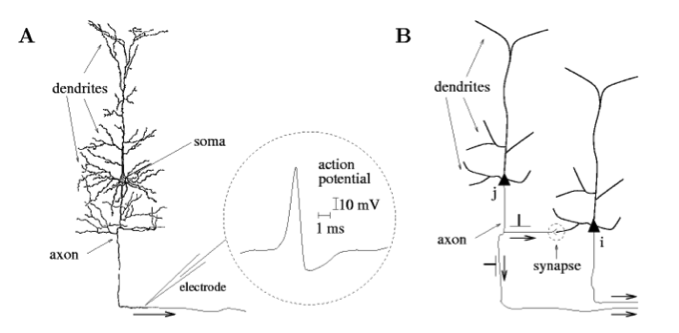
\includegraphics{chapter2/dendrites.png}

\begin{figure}[h!]
  \centering
    \centering
      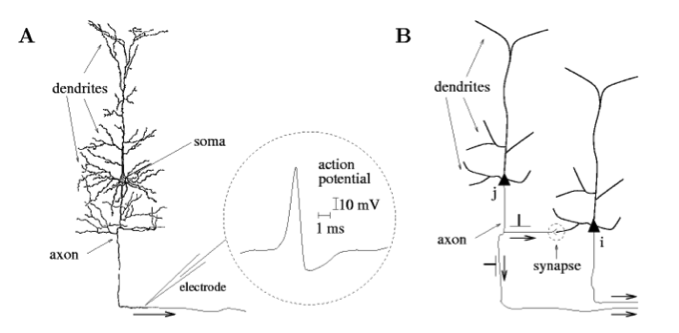
\includegraphics[width=0.5\textwidth]{chapter2/dendrites.png}
  	\caption{A. The inset shows an example of a neuronal action 
		potential. 	The action potential is a short voltage pulse of 
		1-2ms duration and 100mV of amplituted. B. Signal 
		transmition from a presynaptic neuron j to a post synaptic 
		neuron i. The synapse is marked by a dashed circle \cite{gernstbook}.}
	\label{dendrites}
\end{figure}

A living neuron maintains a voltage drop across its membrane. Every cell is surrounded by positive and negative ions. The main ions are K$^{\textrm{+}}$ (Potassium), Cl$^{\textrm{-}}$ (chloride), Na$^{\textrm{+}}$ (sodium) and Ca$^{\textrm{2+}}$ (calcium). In the inner surface of the membrane there is an excess of negative charges and on the outer surface there is an excess of positive charges. Those charges create the membrane potential.

The membrane potential can be calculated from the following equation: Vm=Vin-Vout, where Vin is the negative charges on the inside of the cell and Vout are the positive charges outside of the cell.  When the membrane potential is at the resting state, that is when it is not receiving any input signals, the resting potential Vrest is set to Vin, which is around -60mV to -70mV.

When the neuron receives an input, some of the ion channels of the cell open and others close, resulting in an electrical current flow into the cell, which results in a change of the resting potential Vrest \cite{princNeuron}.

The phenomenon during which the membrane's potential changes exceed the resting potential is called depolarization. The opposite phenomenon is called hyperpolarization. When the depolarization reaches a critical value, also known as threshold, the cell produces an action potential (a spike) \cite{princNeuron}, figure 1.2. If the membrane potential receives an input that causes depolarization or hyperpolarization and after that does not receive any other input, the membrane potential returns slowly to its resting potential.

In the case of the Glial cell the potassium K+ are flowing from the inside of the cell to the outside causing a potential difference called equilibrium potential Ek \cite{princNeuron} . This E$_{\textrm{k}}$ determines the resting membrane potential and can be calculated from the Nerst Equation:


\begin{equation} \label{eq:EK}
	E_k = {RT \over zF} ln {[X]_o \over [X]_i}
\end{equation}
 
Where R is the gas constant, T is the temperature in Kelvin, z is the valence of the ion, F the Faraday constant, [X]$_{\textrm{o}}$ and [X]$_{\textrm{i}}$ are the concentrations of the ion outside and inside of the cell \cite{princNeuron}.  Thus the Vrest for the Glial cell is Vrest = -75mV. The membrane potential will be discussed in the next section when the Hodgkin-Huxley neuron model will be described based on the experiments on the squid giant axon.

\subsubsection{The Action Potential}

As stated before, when the membrane potential reaches a critical value called threshold it emits an action potential, also known as a spike. This is caused by the movement of ions across the membrane through voltage-gated channels \cite{princNeuron}.  The spikes are identical to each other and their form does not change as the signal moves from a presynaptic to a postsynaptic neuron \cite{gernstbook}. The firing times of a neuron are called spike train and it is represented with the following equation: 

\begin{equation} \label{eq:spiketrain}
	Fi=\{t^1_i, t^2_i, ..., t^n_i\}
\end{equation}

The subscript i defines the neuron and the superscript defines the number of the emitted spikes, where n is the most recent emitted spike.

	Directly after the transmission of a spike, the membrane potential goes through a phase of high hyperpolarization under the resting potential and then slowly returns back to the resting potential. During that time, it is not possible to emit a second spike even for strong input signals, that is because the ion channels are open instantly after a spike has been generated \cite{gernstbook}. The minimum time between two generated spikes is called absolute refractory period and the phenomenon where the membrane potential undershoots below the resting potential is known as the spike after potential (SAP), Figure~\ref{sap}.

\begin{figure}[h!]
  \centering
    \centering
      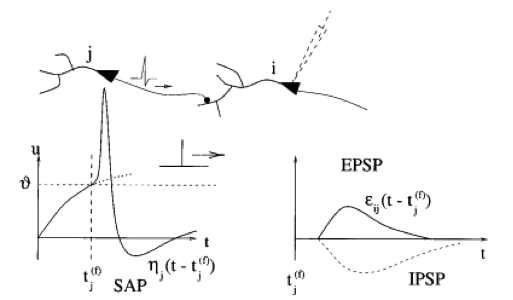
\includegraphics[width=0.5\textwidth]{chapter2/sap.png}
  	\caption{The membrane potential is increased and at time tj(f) the membrane potential reaches the threshold so a spike is emmited \cite{pnn}.}
	\label{sap}
\end{figure}
 
 \subsubsection{The Synapse}

Between the axon of the presynaptic neuron and the dendrite of the postsynaptic neuron there is a small gap, also known as synaptic gap. The operation of the synapse is very complicated and a detailed description is beyond the scope of this review.
 The spike of the presynaptic neuron cannot cross this gap, however, when a spike arrives from the presynaptic neuron to the synapse the gap is filled a fluid that generates a postsynaptic potential (PSP) to the dendrite of the postsynaptic neuron \cite{princNeuron}. This process does not happen instantaneous; there is a small delay generated in that particular synapse.
 
There are two types of postsynaptic potentials. If the generated postsynaptic potential is positive it is called excitatory postsynaptic potential (EPSP) or if the generated postsynaptic potential is negative it is call inhibitory postsynaptic potential (IPSP), Figure~\ref{psp}. An IPSP lowers the membrane potential of the postsynaptic neuron while an EPSP increases it and may cause it to fire a spike.  

\begin{figure}[h!]
	\centering
	\centering
	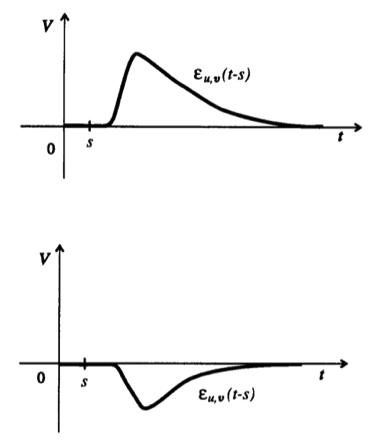
\includegraphics[width=0.3\textwidth]{chapter2/psp.png}
		\caption{Excitatory postsynaptic potential (EPSP) and Inhibitory 
			postsynaptic potential (IPSP) of a biological neuron \cite{Maass97networksof}.}
		\label{psp}
\end{figure}

\subsubsection{Spiking Neuron Models}

Spiking neuron models can be divided into two major categories \cite{gernstbook} based on their level of abstraction: The conductance models and the threshold models. The conductance models simulate the ion channels of the cell, while the threshold models represent a higher level of abstraction where the threshold voltage has a fixed value and the neuron fires every time the membrane potential reaches it.

	There are two additional models that will not be described in this thesis: the compartmental and rate models. The compartmental models will not be discussed due to their complexity and the rate models are actually the sigmoidal neurons that are used in the traditional artificial neural networks of the 2nd generation. Due to their nature, they neglect all the temporal information of the spikes and only describe their activity as spike rates.

In general, Conductance-Based models have been derived from the Nobel prize winners (1963) Hodgkin and Huxley, based on the experiments that they performed on the giant axon squid \cite{hhmodel}. Basically, they describe what happens to the ion channels of the neuron cell. 

\subsubsection{Leaky-Integrate-and-Fire Model}
%%%%%%%
% LIF MODEL START
%%%%%%%

The Leaky Integrate-and-Fire neurons are threshold-fire models that are based on the summation of all contributions of the presynaptic neurons to the membrane potential. If the membrane potential reaches a fixed threshold from below, the neuron will fire and after an axonal delay it will cause neurotransmitter release from the synapses. 

They have been extensively used in large spiking neural networks \cite{Delorme1999989} because of their ease of implementation and the low computational cost.

The basic circuit of the integrate-and-fire model can be seen in Figure~\ref{lif1new}. It consists of a resistor R in parallel with a capacitor C that models the passive patch of the membrane. In addition, a reset mechanism has been added, as a switch that closes when the membrance potential reaches a threshold value from below. 
% A pulse coming from a presynaptic neuron, passes from a low-pass RC filter before it is fed to the postsynaptic neuron. 

\begin{figure}[h!]
\centering
\centering
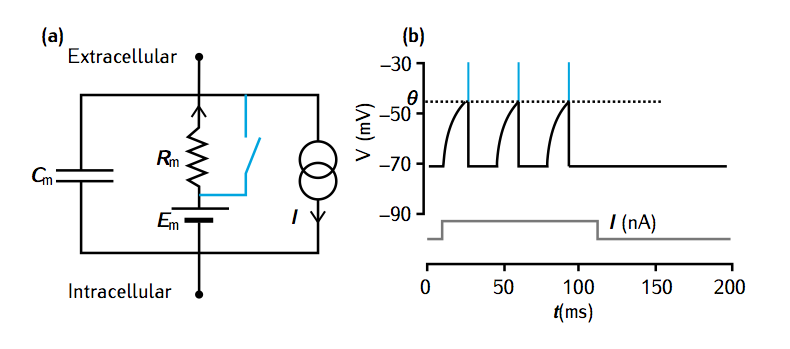
\includegraphics[width=0.7\textwidth]{chapter2/lif1new.png}
	\caption{The Leaky Integrate-and-fire model. (a) The RC circuit diagram of the model. When the membrane potential reaches a threshold voltage ${\theta}$, the neuron is considered to have fired a spike and the switch closes. The aforementioned short-circuit causes the membrane potential to return back to the resting membrane potential E$_{m}$. (b) Response of LIF circuit to current injection. The refractory period can be observed directly after the firing of a spike \cite{sterratt2011principles}.}
	\label{lif1new}
\end{figure}

Using the Ohm's law, the schematic in the Figure~\ref{lif1new} can be described by the following equation:

\begin{equation} \label{eq:lif1}
C_{m} {dV\over dt} =- { {V - E_{m}} \over R_{m}} + I 
\end{equation}

Where C$_{m}$ is the membrance capacitance, R$_{m}$ is the membrane reistance and I is the total current flowing into the cell, which could be from an electrode or from other synapses, see equation \ref{eq:neurotrans}. Furthermore, by setting ${\tau}_{m}$ = RC, the equation \ref{eq:lif1} could be rewritten as:

\begin{equation} \label{eq:lif2}
{\tau}_{m} {dV\over dt} = -V + E_{m} + R_{m}I
\end{equation}

Where ${\tau}_{m}$ is known as membrane time constant. When the membrane potential reaches a predefined threshold ${\theta}$, the neuron fires a spike and the membrane potential is reset to E$_{m}$.\\

The electrical current resulting from the neurotransmitter at time t$_{s}$ is, for t >= t$_{s}$:

\begin{equation} \label{eq:neurotrans}
	I_{syn}(t) = g_{syn}(t)(V(t) - E_{syn})
\end{equation}

Where g$_{syn}$(t) is the synaptic conductance which peaks at $\bar{g}_{syn}$, V(t) is the membrane voltage of the postsynaptic neuron, for conductance-based synapses (COBA) and E$_{syn}$ is the reversal potential of the synaptic conductance. In many cases equation \ref{eq:neurotrans} can be simplified so that synapses can be thought of as sources of current instead of conductance (CUBA), this is done by setting V = V$_{rest}$ in equation \ref{eq:neurotrans}. This simplification is a good approximation for excitatory synapses but not for inhibitory synapses where the inhibitory reversal potential could be close or even above the resting potential \cite{Schutter:2009:CMM:1822639}. The three commonly used equations for the synaptic conductance are the: (a) single exponential decay, (b) alpha function and (c) dual exponential function:

%\begin{subequations}
%\label{eq:synapsess}
%\begin{gather*}
 % g_{syn}(t) = \bar{g}_{syn} exp(-{{t-t_{s}}\over \tau})  \label{singleexp} \\
  %g_{syn}(t) = \bar{g}_{syn} {{t-t_{s}}\over \tau } exp(-{{t-t_{s}}\over \tau})  \label{alfafunc} \\
  %g_{syn}(t) = \bar{g}_{syn} {{\tau_{1}  \tau_{2} }\over {\tau_{1} - \tau_{2} } }   (exp(-{{t-t_{s}}\over \tau_{1} }) - exp(-{{t-t_{s}}\over \tau_{2} })  \label{dualexp}
%\end{gather*} 
%\end{subequations}

\begin{subequations}
\label{eq:synapsess}
\begin{align}
  g_{syn} &= \bar{g}_{syn} exp(-{{t-t_{s}}\over \tau})  \label{singleexp} \\
  g_{syn} &= \bar{g}_{syn} {{t-t_{s}}\over \tau } exp(-{{t-t_{s}}\over \tau})  \label{alfafunc} \\
  g_{syn} &= \bar{g}_{syn} {{\tau_{1}  \tau_{2} }\over {\tau_{1} - \tau_{2} } }   (exp(-{{t-t_{s}}\over \tau_{1} }) - exp(-{{t-t_{s}}\over \tau_{2} })  \label{dualexp}
\end{align} 
\end{subequations}

Finally, a number of variations of the Leaky Integrate-and-Fire have been proposed to model more complex firing patterns such as the firing rate adaptation or bursting (Type II firing). These models are the Quadratic Integrate-and-Fire model and the Exponential Integrate-and-Fire-model \cite{sterratt2011principles}.

%Section~\ref{sec:np} of this paper presents the details of the hardware of the proposed neuromorphic system, including the silicon retina and the SpiNNaker platform.
%The neural network models are defined and tested on Matlab, and the model structures and experimental results stated in Section~\ref{sec:cnn}.
%In Section~\ref{sec:rrs}, the rate-based models are converted into spiking neurons, and real-time live recognition and recorded data experiments are carried out.
%The contribution of this work is summarised and the future directions are provided in Section~\ref{sec:cfw}.
\subsection{Spike Coding}
Dynamic recognition takes advantage of the intrinsic temporal processing of SNNs which are receiving considerable attention for  undertaking vision processing.
Pattern information can be encoded in the delays between the pre- and post-synaptic spikes since the spiking neurons are capable of computing radial basis functions (RBFs)~\cite{hopfield1995pattern}.
Spatio-temporal information can also be stored in the exact firing time rather than relative delays~\cite{natschlager1998spatial}.
Maass~\cite{maass1997networks} has proved mathematically that:
1) networks of spiking neurons are computationally more powerful than the first and second generation of neural network models;
2) a concrete biologically relevant function can be computed by a single spiking neuron, replacing  hundreds of hidden units in a sigmoidal neural net;
3) any function that can be computed by a small sigmoidal neural net can also be computed by a small network of spiking neurons.
\subsection{Rate Coding}

In rate coding the information is encoded into the mean firing rate of the neuron also known as temporal average \cite{gernstbook}:

\begin{equation} \label{eq:lif2}
v = {{n_{sp}(T)} \over T}
\end{equation}

Where T is time window, nsp(T) are the number spikes emitted during the time window. There are three averaging procedures \cite{gernstbook}: Rate as a spike count (average over time), rate as a spike density (average over several runs) and rate as a population activity (average over several neurons).

\subsection{Temporal Coding}

In temporal coding the information is encoded in the form of spike times \cite{Bohte:2004:ENI:990372.990380}. Hopfield \cite{hopfield_pattern_1995} has proposed a method for encoding analogue data into timing of the spikes with respect to an oscillatory pattern of activity. This method has been proven experimentally in the electric fish. In addition, Maass \cite{Maass97networksof} proposed a method of encoding analogue information in the form of firing times. A different approach has been suggested by Wen and Sendhoff \cite{Jin:2007:EMO:1776814.1776856}, where the input neurons encode information directly into spiking times and an additional bias neuron is used as a time reference. Finally, in polychronization \cite{Izhikevich:2006:PCS:1117652.1117653}, proposed by Izhikevich,  the synaptic delays are tuned so that a neuron would respond to particular spatio-temporal patterns of activity.

\subsection{Population Coding}

In population coding a number of input neurons (population) are involved in the analogue encoding and produce different firing times. Bohte et al. \cite{Bohte02unsupervisedclustering} proposed a way of representing analogue input values into spike times using population coding. Multiple Gaussian Receptive Fields (GRF) were used so that the input neurons will encode an input value into spike times, Figure~\ref{codpop1}.  

\begin{figure}[h!]
\centering
\centering
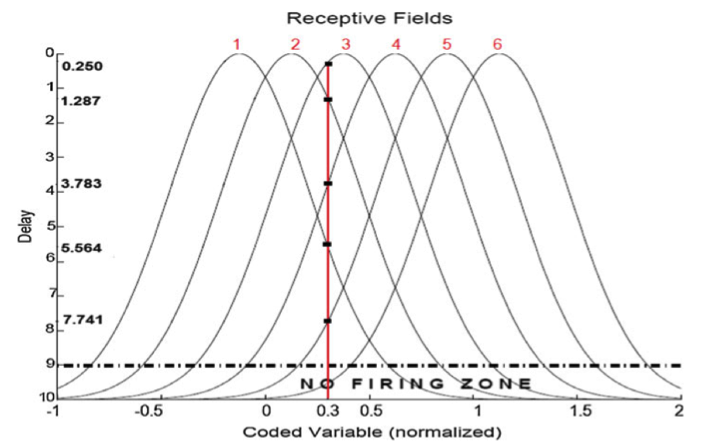
\includegraphics[width=0.7\textwidth]{chapter2/codpop.png}
	\caption{ Encoding with Gaussian Receptive Fields. The horizontal axis represents the real input data, the vertical axis represent the firing times of the input neurons to an input value 0.3 \cite{Meftah:2010:SED:1873252.1873282}. }
	\label{codpop1}
\end{figure}

Firstly the range of the input data has to be calculated. Then the values Imax and Imin, which are the maximum and minimum values of the input data, have to be defined. Furthermore, the number of GRF neurons that are going to be used has to be chosen through the m variable. Lastly, the center of each GRF neuron is calculated from C$_{i}$ while the width of each GRF neuron is calculated by ${\sigma_i}$ \cite{Meftah:2010:SED:1873252.1873282}:

\begin{subequations}
\label{eq:popcod}
 \begin{align}
  C_i = I_{min} +{{(2i-3)}\over 2}    {{(I_{max} - I_{min})}\over m-2} \label{ci} \\
  \sigma_i = {1\over \gamma} {{(I_{max} - I_{min})}\over m-2} \label{si}
 \end{align}
\end{subequations}

Where ${\gamma}$ is constant number usually around 1.5. A threshold value has to be used so that GRF neurons, that are below the threshold, should not fire.  In the example of Figure~\ref{codpop1} the analogue value 0.3 is encoded into firing times of neuron 3 (0.250ms), neuron 2 (1.287ms), neuron 4 (3.783ms), neuron 1 (5.564ms) and neuron 5 (7.741ms). Neuron 6 does not emit a spike because it's below the threshold. 

A different approach to population encoding was proposed by Eliasmith et al. in \cite{Eliasmith02}, where the firing rates of a heterogeneous population of neurons is used to encode an analogue value. Also, the rank-order coding proposed in \cite{Thorpe2001715} encodes an input value based on the order of spikes of a population.  

\subsection{Learning}
In 1949 Hebb formulated the famous Hebb law \cite{Hebb1949}: ''When an axon of cell A is near enough to excite cell B or repeatedly or persistently takes part in firing it, some growth process or metabolic change takes place in one or both cells such that A's efficiency, as one of the cells firing B, is increased''.

Hebb's law is modified so that the weights are updated based on the pre and postsynaptic activity of the neurons, also known as Spike Time Dependent Plasticity (STDP) \cite{gernstbook}.

\begin{figure}[h!]
\centering
\centering
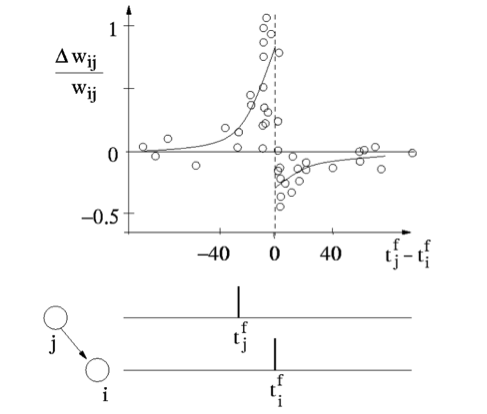
\includegraphics[width=0.7\textwidth]{chapter2/bigpoo.png}
	\caption{ The weights are changing only if the firing times of neurons j and i are close to each other. Data taken from the experiments of Bi and Poo \cite{bigpoo}. }
	\label{bigpoo1}
\end{figure}

In Figure \ref{bigpoo1} neuron j is the presynaptic neuron, neuron i is the postsynaptic neuron and t$_{j}^{f}$ is the presynaptic fire time and tif is the postsynaptic fire time.

Furthermore, Bi and Poo \cite{bigpoo,bipoo2} found out that the synaptic efficacy $\Delta$w$_{ij}$ is a function of the spike times of the presynaptic and postsynaptic neurons. Hence the term Spike Timing-Dependent Plasticity.

	A way to calculate the synaptic weight updates has been proposed by Gerstner et al. \cite{gernstbook} with the use of exponential learning windows:

\begin{equation}
  \Delta W = \left\{ 
  \begin{array}{l l}
    A_{+}exp(s/\tau_{1}) & \quad \text{if $s$ < 0}\\
    A_{-}exp(s/\tau_{2}) & \quad \text{if $s$ > 0}\\
  \end{array} \right.
\end{equation}

Where s = t$_{j}^{(f)}$-t$_{i}^{(f)}$ is the time difference between presynaptic and postsynaptic firing times. The $\tau_{1}$ and $\tau_{2}$ are constants and the A$_{+}$ and A$_{-}$ are used for stability issues in order to cap the weights to a maximum and minimum value, Figure \ref{dw1}. 

\begin{figure}[h!]
\centering
\centering
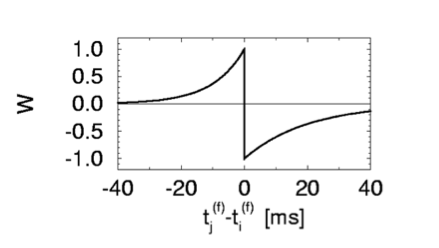
\includegraphics[width=0.4\textwidth]{chapter2/stdpdw.png}
	\caption{ The exponential learning window as a function the difference between the presynaptic and the postsynaptic firing times. A$_{+}$=1, A$_{-}$=-1, $\tau_{1}$=10ms, $\tau_{2}$=20ms \cite{gernstbook}. }
	\label{dw1}
\end{figure}

Numerous methods have been proposed in order to overcome the need of capping the weights to maximum and minimum values for unsupervised learning. For example, the BCM theory, named after the names of the authors ($\bf B$ienenstock, $\bf C$ooper, $\bf M$unro) and it is based on experiments they conducted on neurons in the primary sensory cortex \cite{Bienenstock}. This method uses a sliding threshold mechanism to overcome the saturation of the weights during STDP. However, this method is too computationally expensive thus making it inadequate for large-scale simulations.

\subsection{Successful Applications}
Numerous applications using SNN-based vision processing have been successfully carried out in the past. 
A dual-layer SNN has been trained using Spike Time Dependent Plasticity (STDP) and employed for character recognition~\cite{gupta2007character}. 
Lee et al.~\cite{6467270} have implemented direction selective filters in real time using spiking neurons, considered as a convolution layer in the model of a so called CNN~\cite{camunas2012event}. 
Different features, such as Gabor filter features (scale, orientation and frequency) and shape can be modelled as layers of feature maps. 
The similar behaviours have been found in the primary visual cortex (V1) in the visual pathway~\cite{rehn2007network} as the foundation for higher level visual process e.g. object recognition.
Rank order coding, as an alternative to conventional rate-based coding, treats the first spike as the most important and has been successfully applied to an orientation detection training process~\cite{delorme2001networks}. 
Nengo~\cite{eliasmith2011nengo} is a graphical and scripting based software package for simulating large-scale neural systems and has been used to build the world's largest functional brain model, Spaun~\cite{eliasmith2012large}. 
An FPGA implementation of a Nengo model for digit recognition has been reported~\cite{naylor2013managing}. 
Deep Belief Networks (DBNs), the 4th generation of artificial neural network, have shown great success in solving classification problems. 
Recent study~\cite{o2013real} in this area has mapped an offline-trained DBN onto an efficient event-driven spiking neural network for digit recognition tasks with resounding success.





\section{Platforms}
\label{sec:plt}
The outline of the platform is illustrated in Figure~\ref{fig:SysOverViewa}, where the hardware system is configured, controlled and monitored by the PC.
%Figure~\ref{fig:SysOverViewb} shows the combined hand posture recognition system; 
The jAER~\cite{delbruck2008frame} event-based processing software on the PC configures the retina and displays the output spikes through a USB link.
The host communicates to the SpiNNaker board via Ethernet to set up its runtime parameters and to download the neural network model off-line.
It visualises~\cite{6252490} the spiking activity of the network in real-time.
The photograph of the hardware platform, Figure~\ref{fig:SysOverViewb}, shows that the silicon retina connects to the SpiNNaker 48-node system via a Spartan-6 FPGA board~\cite{galluppi2012real}.
%, which was also applied to a sound localisation system.


\begin{figure}
\centering
	\begin{subfigure}[t]{0.6\textwidth}
		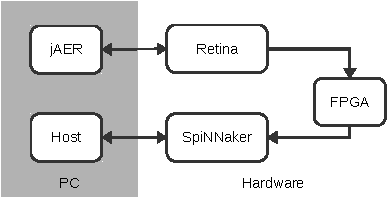
\includegraphics[width=\textwidth]{pics/outline.pdf}
	    \caption{Outline of the platform.}
	    \label{fig:SysOverViewa}
	\end{subfigure}
	\\
	\begin{subfigure}[t]{0.6\textwidth}
		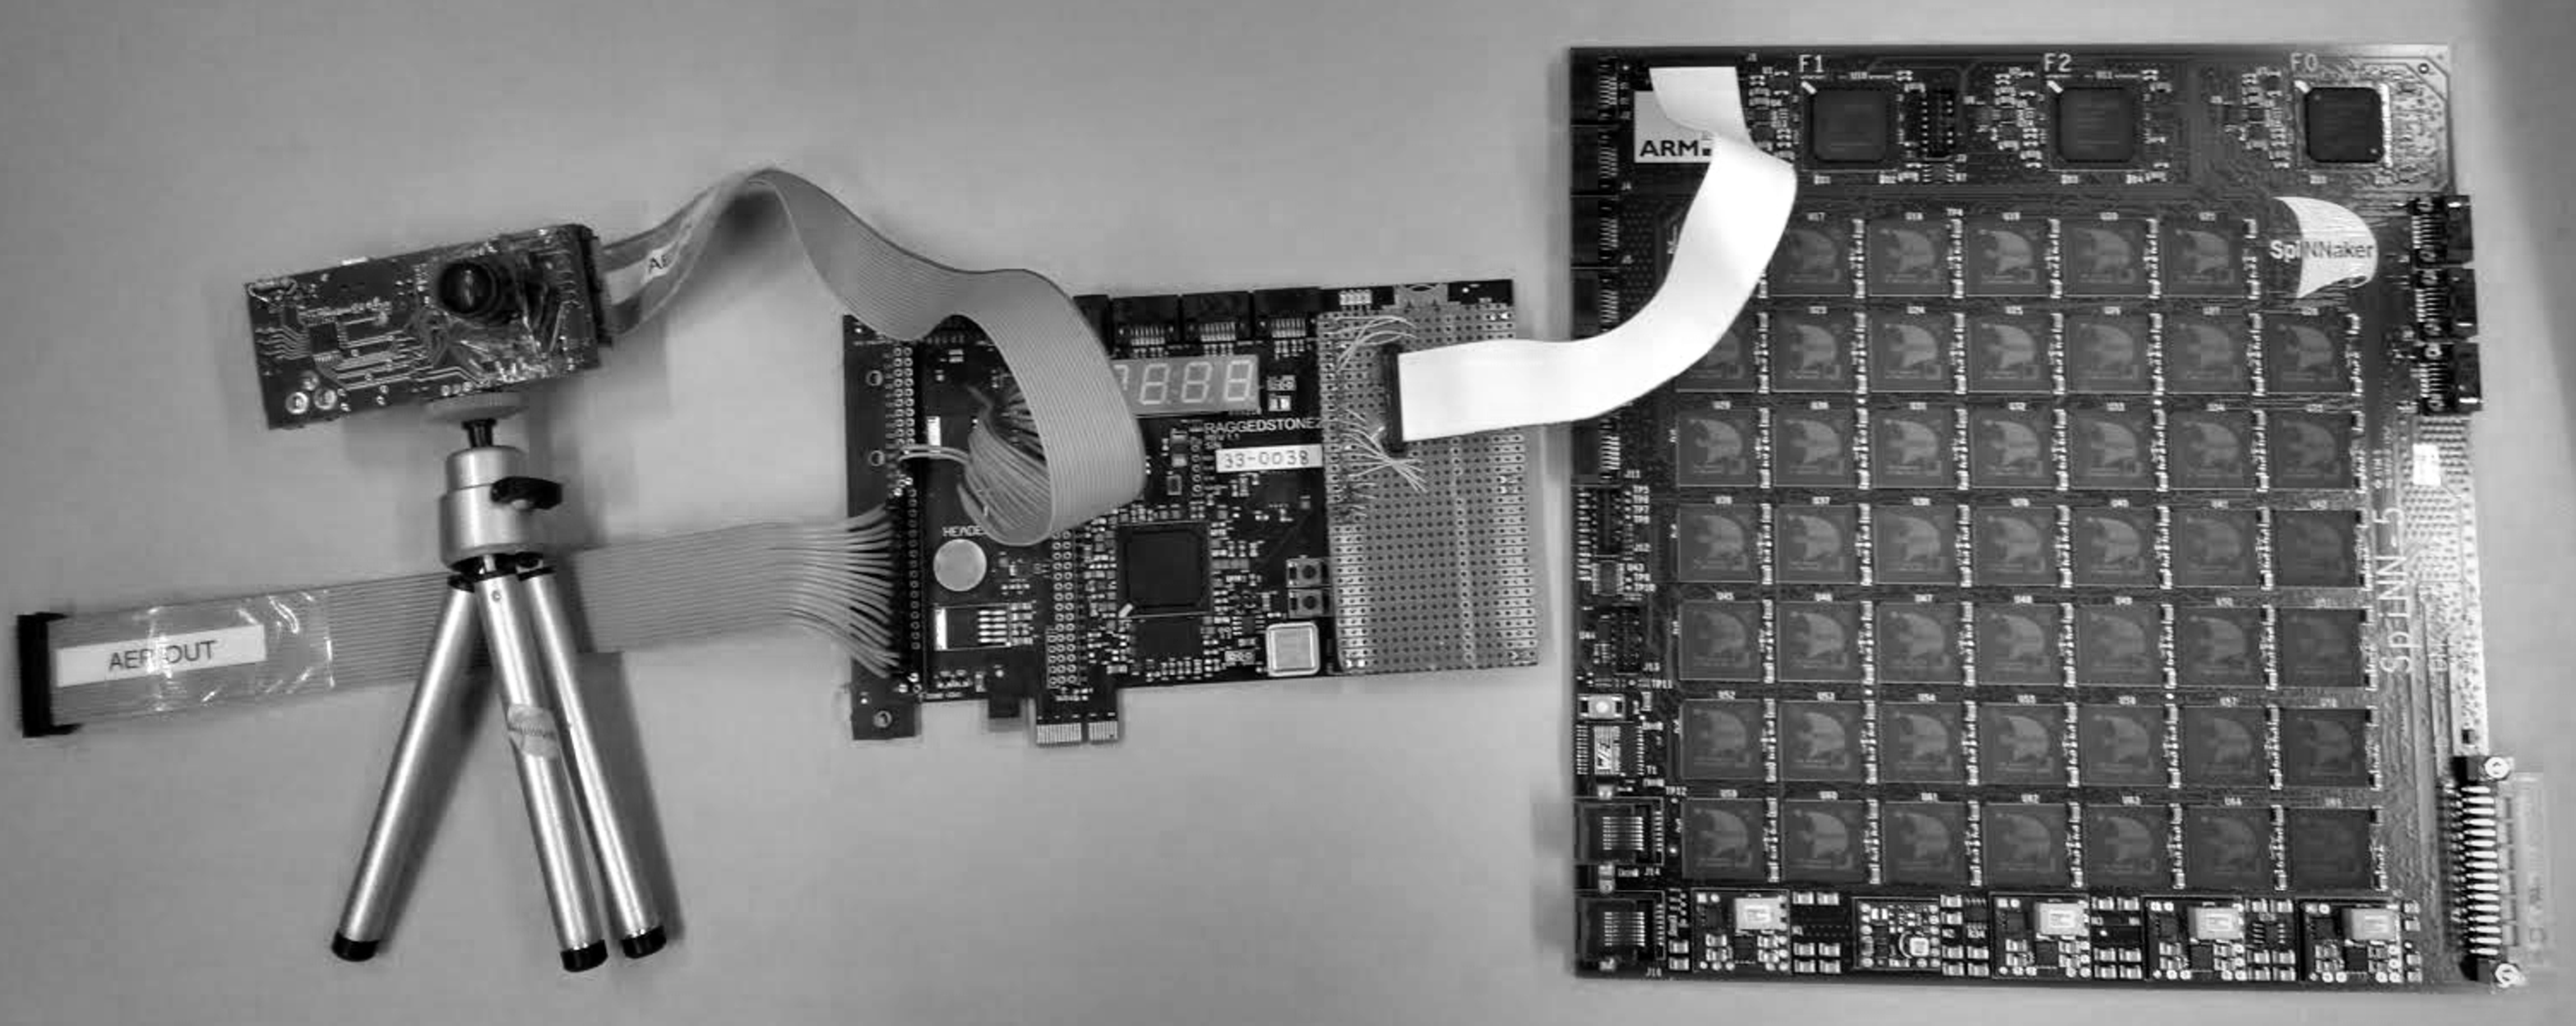
\includegraphics[width=\textwidth]{pics/outline2.pdf}	    \caption{Picture of the hardware platform. From left to right: a silicon retina, a FPGA board, and a 48-node SpiNNaker system.}
	    \label{fig:SysOverViewb}
	\end{subfigure}	

\caption{System overview of the dynamic hand posture recognition platform. 
%The silicon retina connects to the SpiNNaker system through an FPGA board. 
%Spikes from the retina are streamed to the SpiNNaker system through this Spartan-6 FPGA board.
%The jAER software configures the retina and displays its outgoing spikes through the USB connection.
%The host sets up the runtime parameters off-line and downloads the network model to the SpiNNaker system.
}
\label{fig:SysOverView}
\end{figure}


\subsection{Vision Processing Front-ends}
The visual input is captured by a DVS silicon retina, which is quite different from conventional video cameras.
Each pixel generates spikes when its change in brightness reaches a defined threshold.
Thus, instead of buffering video into frames, the activity of pixels is sent out and processed continuously with time.
The communication bandwidth is therefore optimised by sending activity only, which is encoded as pixel events using Address-Event Representation (AER~\cite{lazzaro1995multi}) protocol.
The level of activity depends on the contrast change; pixels generate spikes faster and more frequently when they are subject to more active change.
The sensor is capable of capturing very fast moving objects (e.g., up to 10 K rotations per second), which is equivalent to 100 K conventional frames per second~\cite{lenero20113}.

\subsection{SNNs Back-ends}
The SpiNNaker project's architecture mimics the human brain's biological structure and functionality. 
This offers the possibility of utilizing massive parallelism and redundancy, as the brain, to provide resilience in an environment of unreliability and failure of individual components.

In the human brain, communication between its computing elements, or neurons, is achieved by the transmission of electrical `spikes' along connecting axons. 
The biological processing of the neuron can be modelled by a digital processor and the axon connectivity can be represented by messages, or information packets, transmitted between a large number of processors which emulate the parallel operation of the billions of neurons comprising the brain.

The engineering of the SpiNNaker concept is illustrated in Figure~\ref{fig:sysdia} where the hierarchy of components can be identified. 
Each element of the toroidal interconnection mesh is a multi-core processor known as the `SpiNNaker Chip' comprising 18 processing cores. 
Each core is a complete processing sub-system with local memory.
It is connected to its local peers via a Network-on-Chip (NoC) which provides high bandwidth on-chip communication and to other SpiNNaker chips via links between them. 
In this way massive parallelism extending to thousands or millions of processors is possible.

\begin{figure}
\centering
	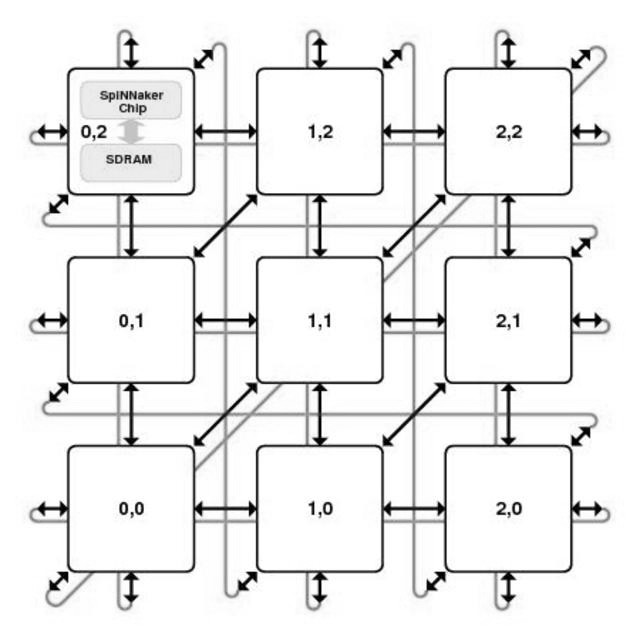
\includegraphics[width=0.8\textwidth]{pics/mesh_ctiff.jpg}
	\caption{SpiNNaker system diagram.
	Each element represents one chip with local memory.
	Every chip connects to its neighbours through the six bi-directional on-board links. }
	\label{fig:sysdia}
\end{figure}

%The knowledge content and learning ability of the brain is generally thought to be embodied in its evolvable interconnection pattern.
%This structure routes a spike generated by one neuron to others which are interconnected with it via axons and these interconnections are modified and extended as a result of learning processes.
%
%In SpiNNaker a packet router within each multi-core processor controls the neural interconnection. 
%Each transmitted packet represents a spike and simply identifies its source neuron.
%This is used by routers to identify whether a packet should be routed to a processor core, or should be routed on to one of the six adjacent chips connected to it as part of the overall SpiNNaker network.

The `103 machine' is the name given to the 48-node board which we use for the hand posture recognition system, see Figure~\ref{fig:48node}.
It has 864 ARM processor cores, typically deployed as 768 application, 48 monitor and 48 spare cores. 
%The `103 machine' requires a 12V 6A supply. 
%The control interface is via two 100Mbps Ethernet connections, one for the board management processor and the second for the SpiNNaker array. 
%There are options to use the nine on-board 3.0~Gbps high-speed serial interfaces (using SATA cables, but not necessarily the SATA protocol) for I/O; 
%this will require suitable configuration of the on-board FPGAs that provide the high-speed serial interface support. 
The boards can be connected together to form larger systems using high-speed serial interfaces. 

%\begin{figure}
%\centering
%	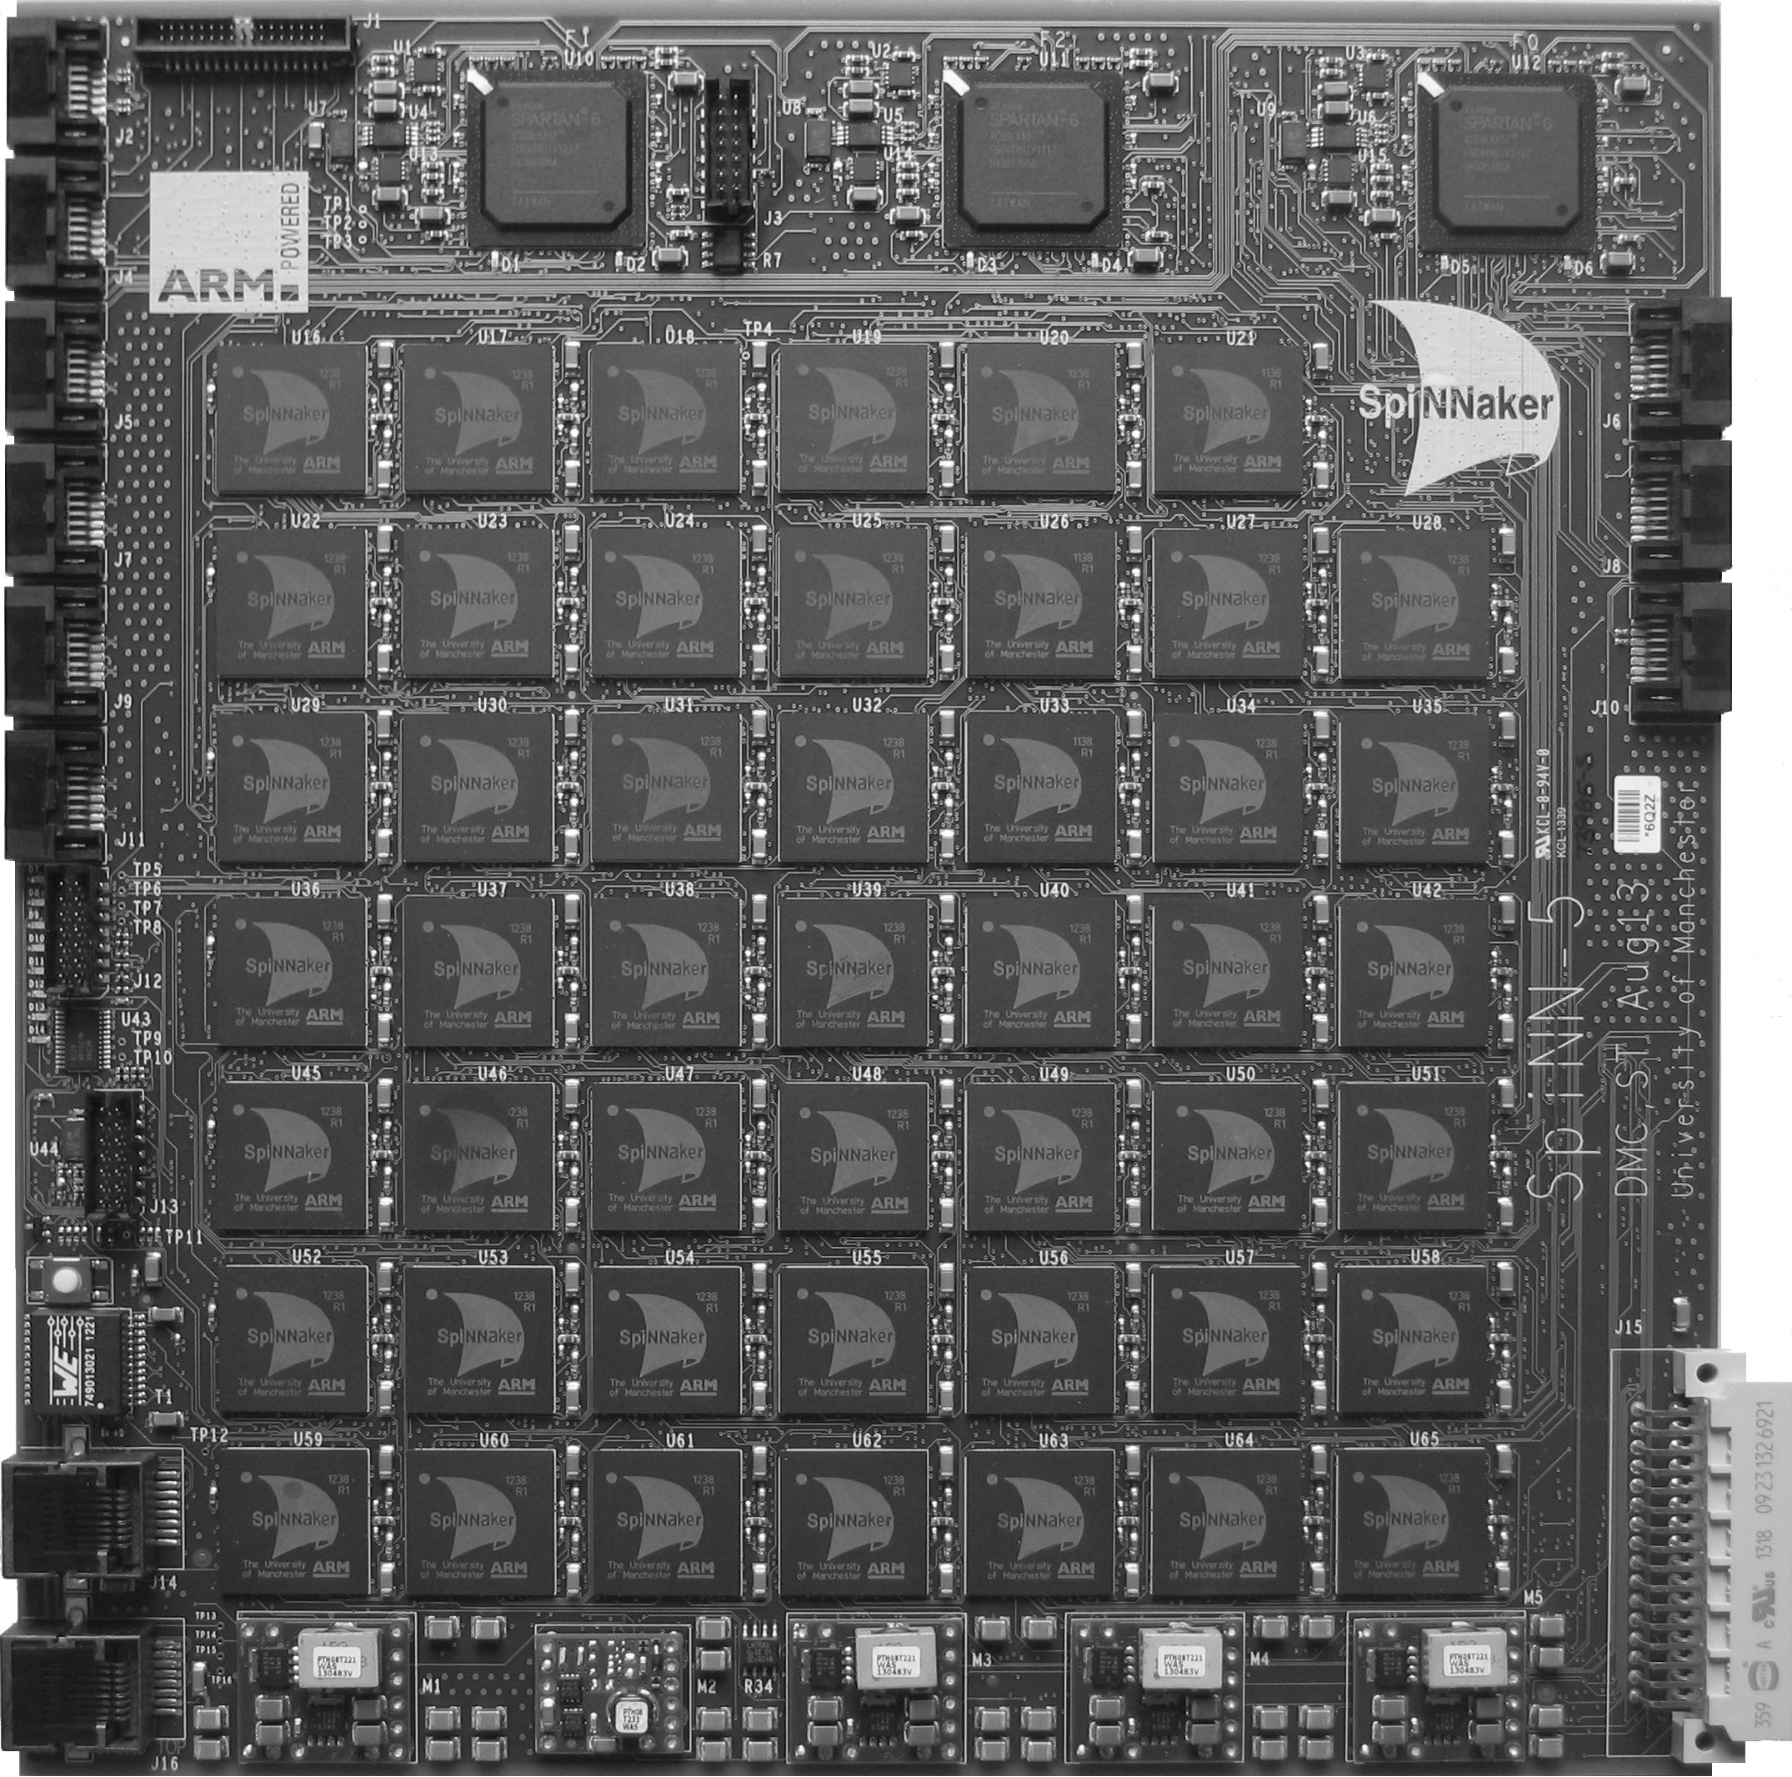
\includegraphics[width=0.6\textwidth]{pics/SpiNN5.pdf}
%	\caption{`103 Machine' PCB}
%	\label{fig:48node}
%\end{figure}

\subsection{SpiNNaker distinguishing features}
Spikes from the silicon retina are injected directly into SpiNNaker via a SPARTAN-6 FPGA board that translates them into a SpiNNaker compatible AER format~\cite{appnote8}. 

From a neural modelling point of view, interfacing the silicon retina is performed using pyNN~\cite{davison2008pynn}. 
The retina is configured as a spike source population that resides on a virtual SpiNNaker chip, to which an AER sensor's spikes are directed, thus abstracting away the hardware details from the user\cite{galluppi2012real}.
Besides the retina, we have successfully connected an AER based silicon cochlea~\cite{5537164} to SpiNNaker for a sound localisation task~\cite{6706931}.

